% !TEX root = ../main.tex
\chapter{Background}\label{ch:chapter2} % For referencing the chapter elsewhere, use \ref{Chapter1}
%
%%----------------------------------------------------------------------------------------
%
To start with, we bring up what is video coding, why it is needed, and
its challenges.
Next we discuss what is deep learning, the history of deep learning and how
it works for vision tasks.
Furthermore, we introduce how we plan to apply deep learning to optimize video
coding and why it should work.
Lastly, a survey of related works on the topic of video coding is presented.

%3D Video applications are attracting more interests
%%----------------------------------------------------------------------------------------
%
\section{Video Coding}\label{sec:video-coding}
Video playback is the most straightforward way for human to perceive dynamic
scenes which exist across a period of time.
More than half of the neurons in human brains are born to process the visual
information supplied by human eyes.
It becomes effortless for human to know what is going on in
video playback.
Videos are made up of consecutive sets of image frames, which in turn
are made up of pixel matrices.

Most of the time videos need to be stored for future use.
In 1950s, video tapes were employed to store videos.
Video tape is able to serve eight to twelve years
before the quality of the stored video starts to degrade.
In 1970s, laser disc appeared in the market as an alternative of video tapes.
Start from laser disc, the video storage started its new era in digital world.
In 1990s, DVDs were released into the market.
Data is stored in spiralling tracks on the disc.
A laser beam can be utilized to read the data.
In addition, hard drives, flash drives and SD cards were also starting to
become popular in the late 90s.
Nowadays, the cloud storage is very common in daily lives.
It is capable of storing data on the servers which are
accessible from any devices via internet connections.

Although so many formats are available for video storage, they share a common
feature: the more storage you use, the more extravagant it will be.
Taking the cloud storage as an example,
Google Cloud is one of the most popular cloud services.
It provides cloud storage with a price
of \SI{0.026}[\$]{} per GB/month~\parencite{RN202}
(this price appears on 21 Nov 2017, it may change in the future).
If there is a video 
(120 frames per second, 
\(4096\times2160\) resolution, 
8 bits per RGB component)
to be stored without
any compression in Google Cloud,
we need to pay a monthly fee of
\((4096\times2160\times120\times60\times90\times3\times0.026)/(1024\times1024\times1024) \approx 416.47\) \$.
Without doubt, this figure is relatively not acceptable for the purpose of
video storage.
High compression is needed to store the videos in a practical way.

From the other perspective, let us take the bandwidth into consideration.
To deliver the uncompressed 4K video which has been mentioned in
the previous paragraph, we need a bandwidth of
\((4096\times2160\times120\times3)/(1024\times1024\times1024) \approx 2.97\) Gigabytes per second.
The maximum bandwidth of Wireless 802.11ac, which is one of the common
internet access technologies, is 1.3 Gigabytes per second~\parencite{RN203}.
Apparently, the wireless connection is not able to deliver such kind of
4K videos.
High compression is desired to deliver the video on the internet.

Despite the fact that raw videos usually contain a large amount of data,
a lot of redundancies exist.
For every video sequence, two types of redundancies are ubiquitous: spacial
redundancy and temporal redundancy.
Video coding technologies are taking advantages of those redundancies to
achieve efficient compression for video data.
Many of the useful video coding technologies have been adopted by the
international video coding standards, such as MPEG-4, H.264, H.265, etc.

Figure~\ref{fig:video-std-brief-history} shows the brief history of
the video coding standards.
\begin{figure}
    \centering
    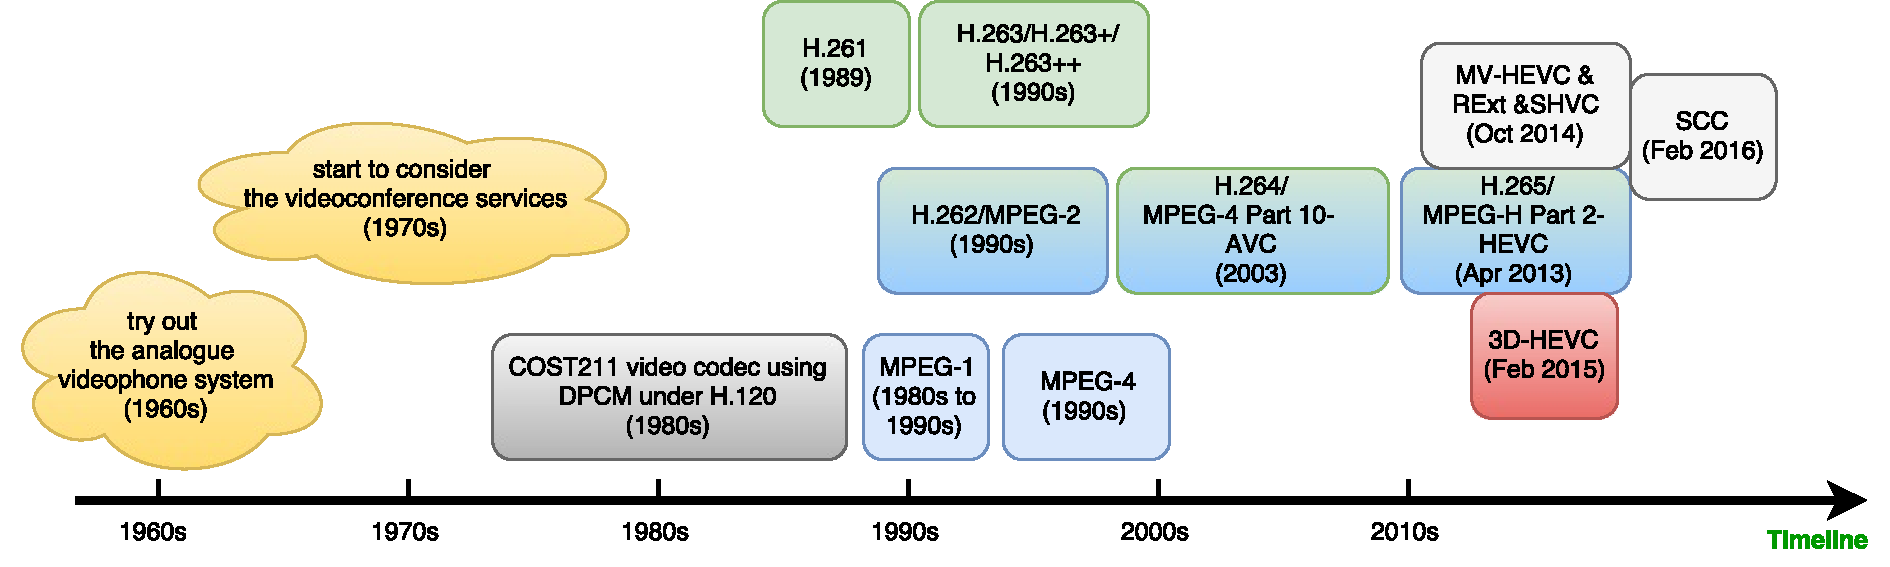
\includegraphics[width=\textwidth,height=\textheight,keepaspectratio]{Figures/video-std-brief-history.pdf}
%        \decoRule
    \caption[The brief history of the video coding standards]
    {The brief history of the video coding standards}\label{fig:video-std-brief-history}
\end{figure}
In 1980s, the COST211 video codec, which was built on top of Differential
Pulse Code Modulation (DPCM), was standardized under H.120 standard by CCITT
(now known as ITU-T).
In late 1989, the H.261 was completed and its success marked a milestone for
video coding at low bit rate with fairly good quality~\parencite{RN181}.
The Motion Picture Experts Group (MPEG) kicked off the exploration of video
storage, such as CD-ROMs.
Their objective was to achieve a competitive performance with cassette
recorders in terms of compression of videos wherein rich motions can be found.
The framework of H.261 was used to start the codec design of MPEG-1.
MPEG-2 is the successor after MPEG-1.
It features high capabilities when handling video with
high bitrate and high resolution.
In MPEG-2, the encoder is allowed to make its own decision on the
the number of bi-directionally predicted pictures according to a
suitable coding delay.
ITU-T found this technique applicable to telecommunication applications, as
a result MPEG-2 has been adopted as H.262 for telecommunications.
Right after the MPEG-2 standard, MPEG-3 was designed mainly for coding of
high definition videos.
However, MPEG-3 was discarded due to the versatility of MPEG-2, which
can be used to encode video of any resolution.
In the late 1998, MPEG-4 was introduced as a standard to define compression of
both audio and visual digital data.
Later on MPEG-4 was divided into several parts during its continuously evolving.
Among its sub-parts, MPEG-4 part 10 (a.k.a.\ Advanced Video Coding) is mainly
for video compression.
With the rising popularity of high definition videos, the new standard
termed High Efficiency Video Coding (HEVC) for compressing videos in a more
efficient way comparing with previous standards, such as H.264/AVC, has
emerged under the efforts from the Joint Collaborative Team on Video
Coding (JCT-VC).
In the meanwhile, five extensions of the HEVC standard, comprising
Format Range Extension (RExt), Scalability Extension (SHVC),
Multi-view Extension (MV-HEVC), 3D Extension (3D-HEVC),
and Screen Content Coding Extension (SCC), have been finalized
from 2014 to 2016 for fulfilling extra requirements in various video coding
scenarios.

In this work, we focus on depth map coding in 3D-HEVC\@.
DC mode, PLANAR mode, 33 angular modes and depth modeling modes 
have been embraced in
depth map coding tools in 3D-HEVC\@.
The DMM1 mode introduces a huge increase for the encoding time of 3D videos.
Acceleration of depth map coding is needed.

\section{Deep Learning}\label{sec:deep-learning}
Deep learning is one of the approaches for representation learning
(a.k.a.\ feature learning), which is essentially a method to
learn from data.
Numerous layers of computational units together with appropriate activating
mechanism comprise the basic architecture for deep learning.
Multitudinous data sets are needed for those computational architectures
to learn data abstractions
for tasks such as image classification, speech recognition,
object detection, etc.
Each layer learns a level of abstraction from the data sets using
back-propagation algorithm~\parencite{RN96}.
Making use of those learned abstractions, the computational models are
able to solve complicated problems which are typically non-linear and normally hard
to solve by using specific rules that are designed by human experts in advance.

Deep learning has attracted wide attention from all over the world
in recent years, not only because of the great achievements it has
made in various application scenarios, but also due to the promise of an
intelligent future it gives.
Such a learning methodology makes people believe that 
the formation of wise machines, which they have long
dreamed to possess, is possible.
The growing data accessibility provides rich datasets for computational
models to adjust their internal weights and bias until their
predictions will have low error rate.
On the other hand, the devices for computation are relatively
affordable than in the previous years. 
With the help of those devices,
accelerations of deep learning have been achieved.
Consequently a bunch of time consuming deep learning architectures 
can be explored within an acceptable range of time.

In the ILSVRC-2012 competition~\parencite{RN205}, AlexNet~\parencite{RN65}
received the championship with the 15.3\% top-5 error rate comparing to
26.2\% error rate achieved by the runner-up.
Such a large margin of error rate claimed a breakthrough in
object recognition history.
Since then, both academia and industry started to try out deep learning
at a blistering pace, which in turn result in an increase of 
the submissions to ILSVRC-2013, in which ZF Net~\parencite{RN66}
was the winner.
It fine-turned the architecture of AlexNet and
gorgeous visualizations of trained models were presented.
Both AlexNet and ZF Net are of the same structure which is built up
by simply stacking computational layers while GoogLeNet~\parencite{RN60}
is composed of Inception
modules.
This new architecture was the most successful candidate in ILSVRC-2014.
It not only reached a new height of object recognition but also 
started the optimization of the computational resources inside network by design.
It consists of 22 layers, which was deeper than all the previous
networks in ILSVRC\@.
However, it was still not deep enough.
In ILSVRC-2015, Residual Neural Network (ResNet)~\parencite{RN67} with
152 layers won the championships in all the five main tracks.
ResNet introduced a brand new notion into the neural network architecture
named identity mapping.
It is implemented by shortcut connections which prevent the degradation of
training precision when the network goes deeper.
Besides, the converging speed of ResNet is faster than the network built up
with Inception modules when both contain similar size of learnable parameters.

Despite the fact that neural networks built up from Inception modules
converge slower than those built up from ResNet modules, it is still
worth it for a brief review of the valuable insights residing in
the Inception networks.
A typical incarnation of the first generation of Inception networks is named
GoogLeNet~\parencite{RN60}.
It was intricately carved with a responsibility to win computer vision
tasks in ILSVRC-2014, on which it performed better than all the other
deep neural network architectures.
The philosophical reflections, which intended to serve as guidelines
for the construction of Inception networks, are highlighted below.
Two major downsides of enlarged neural networks have been discussed
in~\parencite{RN60}.
One is the higher chance of overfitting while the other is
the strikingly increased requirements of computational resources.
To overcome those drawbacks, based on the new ideas 
about how to construct reasonable architectures of
neural networks in~\parencite{RN207}, new experiments orienting 
sparse network architecture have been conducted.
One year later after GoogleNet hold the championship of ILSVRC-2014,
an approach named Batch Normalization~\parencite{RN61} was
proposed by Google researchers to accelerate and ease the
training of deep neural networks.
The core idea behind Batch Normalization is to normalize
the inputs to each layer for every batch of training data.
More importantly, normalization
essentially is matrix multiplications followed by adding biases.
Due to this observation, the Batch Normalization, which is implemented 
as additional layers, has been made part of
the network architecture.
This rather novel method started a new chapter for the training of deep
neural networks.
With the adoption of Batch Normalization, higher learning rates no longer
impede the convergence of the deep networks, oppositely faster
training speed, which can achieve a
better accuracy of prediction with considerably less time, is brought to scene.
Additionally, in some cases, it can even replace the Dropout~\parencite{RN70}
which is an effective method to prevent overfitting.
The incorporation of Batch Normalization into the first generation of
Inception network architecture result in the formation of Inception-v2 which
improved the best accuracy on ImageNet classification with less training steps.
%more advanced accuracy on ILSVRC 2012
%classification challenge validation set.
In the same year, Inception-v3~\parencite{RN62} joined the party, 
the objective of which was
to effectively leverage the power of additional computation by factorizing
to smaller size convolutions and regularizing the classifier layer with
the estimation of minor effect of label-dropout in the training process.
The network architectures were scaled up in Inception-v3, which consequently
imposed higher requirements of available computational resources.
With the ResNet~\parencite{RN67} stealing the show in ILSVRC-2015,
the influence of the
identity mapping in residual units on learning process
has been investigated in~\parencite{RN63}.
The filter concatenation stage of Inception-v3 was replaced using shortcut
connections which effectuated the layout of a new model 
named Inception-ResNet-v1.
A more advanced version, which was named Inception-ResNet-v2, has a larger
network size than the first version.
Besides the mixed architectures of Inception-ResNet, a pure Inception
incarnation named Inception-v4 was also presented with comparison to
Inception-ResNet-v2.
Both Inception-v4 and Inception-ResNet-v2 have significant gain of performance
mainly benefiting from the enlarged size of network.

\section{Related Work}\label{sec:related-work}
In this section, the prior arts working on video
coding optimizations are reviewed.
The differences between this work and others
are compared.

Before the occurrence of Depth Modeling Mode (DMM) and
View Synthesis Optimization (VSO) in~\parencite{RN208}, a lot of literature
on depth map coding, which have been published, are mainly
focusing on improving the effectiveness of depth map coding.
Based on the observation that the depth map is characterized by vast
smooth regions, which are separated by sharp edges, 
an algorithm to effectively
encode homogeneous regions has been proposed in~\parencite{RN120}.
It improves coding performance for depth map by copying pixel values for
homogeneous blocks from values of neighboring reference pixels.
In~\parencite{RN123}, Depth Lookup Table (DLT) has been proposed for
encoding the depth map in 3D-HEVC standard.
It offers the benefit of 1.3\% bitrate reduction.
To further improve the coding performance for depth map, more
effectual tools for depth map coding are needed.
Depth Modeling Mode (DMM) and View Synthesis Optimization (VSO) are proposed
in~\parencite{RN208}.
VSO provides 17\% bitrate reduction in average, while DMM provides 6\% 
average savings on bitrate.
Although the introductions of DMM and VSO bring the effectiveness of
depth map coding into a new level, the computational complexity increases
a lot due to the complex nature of VSO\@.
Consequently, the time cost of depth map encoding becomes fairly expensive.

The computational complexity of depth map coding
raised the question of whether it is possible to reduce the computational
complexity for saving encoding time.
In~\parencite{RN76}, a fast wedgelet searching scheme achieves significant
reduction for computational complexity with minor decrease on BD performance.
It takes advantage of the results from
Sum of Absolute Transform Difference (SATD) to reduce the wedgelet searching
candidates.
Rough RD cost from Rough Mode Decision (RMD) is used as mode selection threshold
in~\parencite{RN90} to speed up the bi-partition modes decision.
A two-step fast searching approach for wedgelet partition
appears in~\parencite{RN126}.
It features a coarse search in conjunction with a further refinement step.
Another fast approach for wedgelet searching~\parencite{RN79}
is to make use of Most Probable Mode (MPM) to reduce wedgelet
searching candidates.
Since intra angular modes will lead to ringing artifacts
when they are utilized for depth map coding, the idea of skipping intra
angular prediction by making use of edge detector is shown in~\parencite{RN89}.
Bayesian classifier is used in~\parencite{RN102} to alleviate the computational
complexity of intra mode decision in 3D-HEVC\@.
The optimal mode of parent prediction unit (PU)
in the hierarchical quad-tree coding structure 
has been utilized to select
the mode for child prediction unit (PU) in~\parencite{RN131}, 
and early decision for segment-wise DC coding is used together 
to achieve faster depth intra coding.
Edge classification in Hadamard transform domain is used in~\parencite{RN86}
to skip the DMM decision process conditionally.
The minimum RD cost of the candidate from full-RD searching list is taken
as the threshold to bypass DMM decision in~\parencite{RN93}.
Most probable region for DMM1 mode decision is identified with the help
of sharp edges in~\parencite{RN209}, and DMM3 is skipped when depth
prediction unit (PU) does not match with co-located texture counterpart.
Variance is utilized in~\parencite{RN210} to estimate the most promising
sub-region for DMM1.
Corner point is used for fast quad-tree decision of depth intra coding
in~\parencite{RN211}.
Variance distribution is studied in~\parencite{RN111}, based on which the
method termed Squared Euclidean distance of variances (SEDV) is
proposed to substitute the long-standing View Synthesis Optimization (VSO)
process.
Besides, a new scheme termed probability-based early depth intra mode
decision (PBED) is employed to skip modes and the RD cost in
Rough Mode Decision (RMD) is used to terminate
segment-wise depth coding (SDC)~\parencite{RN123}
as early as possible.
The correlation between depth map and texture view is explored
in~\parencite{RN94} to palliate the sophistication of
compression for depth map.
In~\parencite{RN212}, comparing RD cost with pre-calculated threshold for fast
intra mode decision together with early decision for the CU depth are used
to accelerate the encoding.
Making use of RD cost results of the angular modes, only the most promising
DMMs are evaluated in~\parencite{RN87} and, moreover, an innovative
method using golden ratio to further improve the
depth map coding is proposed.
The characteristics of depth map are studied in~\parencite{RN91},
as a result only four conventional intra modes are used for
depth map intra coding and only six directions are used in DMM1 searching.
Block edge along with the border gradient are used together
in~\parencite{RN114} to surge the speed of depth map coding.
Information of neighboring blocks and threshold which is derived from
lots of experiments are used in~\parencite{RN85} for improving depth
map coding.

Despite the aforementioned works which are using heuristic approaches,
machine learning approaches are also applied for video coding optimization.
In~\parencite{RN74}, the decision for the depth of coding units (CUs)
in High Efficiency Video Coding (HEVC) is modeled as a classification
problem which can be solved by machine learning approach.
A shallow convolutional neural network (CNN) is
used in~\parencite{RN78} to determine coding unit depth in
High Efficiency Video Coding (HEVC) while
in~\parencite{DBLP:journals-corr-abs-1710-01218}, a deeper convolutional
neural network together with long- and short-term memory (LSTM) network
are employed to address the same issue.
In additional to the works which are targeting the
coding unit depth decision using machine learning approaches, it is found
in~\parencite{RN73} that deep learning is used for the intra mode
selection in Screen Content Coding (SCC)
Extension of High Efficiency Video Coding (HEVC).

The researching focus in this thesis is the same as~\parencite{RN73}.
However, there are three significant differences between two works.
Firstly, the network in this thesis, which consists of 32 layers, is
much deeper than the 4-layer network in~\parencite{RN73}.
Secondly, unlike the server-client setup in~\parencite{RN73}, we have
managed to integrate the learned models into the codebase of \(HTM16.2\).
Executable binary can be obtained which is totally self-contained in the
sense that they are not relying on the remote server to do the prediction,
just the binary itself is capable of doing prediction
for mode selection in depth maps.
Lastly, in this work, deep learning is for depth map coding in
Three Dimension Extension of High Efficiency Video Coding (3D-HEVC)
while in~\parencite{RN73} the learning is for Screen Content Coding (SCC)
Extension of High Efficiency Video Coding (HEVC).
% 